\documentclass[titlepage, 12pt]{article}

\usepackage{framed}
\usepackage{enumitem}
\usepackage{geometry}
\geometry{
  letterpaper,
  margin=1in,
}
\usepackage{graphicx}
\graphicspath{{./images/}}
\usepackage{float}
\usepackage[page]{appendix}

\title{SE 2XB3 Group 4 Report 1}
\author{
  Huang, Kehao \\
  400235182 \\
  \texttt{huangk53@mcmaster.ca} \\
  L01
  \and
  Jiao, Anhao \\
  400251837 \\
  \texttt{jaoa3@mcmaster.ca} \\
  L01
  \and
  Ye, Xunzhou \\
  400268576 \\
  \texttt{yex33@mcmaster.ca} \\
  L01
}
\date{22 January 2021}

\begin{document}

\maketitle{}

\section*{Team Contract}
\label{sec:contract}

\begin{itemize}
\item We will primarily be using Discord to communicate.
\item All members must respond to messages which they are mentioned in within 2
  hours.
\item During 3:30pm--5:30pm on Mondays, all members must present in a Discord
  meeting to prepare for the lab on Tuesday.
\item During the assigned lab period on Tuesdays 8:30am--11:20am, all members
  must present in a Discord meeting to work on the lab.
\end{itemize}

\subsection*{Signatures}

\bigskip{}

\begin{minipage}[t][4em][t]{0.33\linewidth}
  
\includegraphics[width=0.8\linewidth]{anhao-signature}
  \centering
  Anhao Jiao
\end{minipage}
\begin{minipage}[t][4em][t]{0.33\linewidth}
  
\includegraphics[width=0.8\linewidth]{kehao-signature}
  \centering
  Kehao Huang
\end{minipage}
\begin{minipage}[t][4em][t]{0.33\linewidth}
  
\includegraphics[width=0.8\linewidth]{xunzhou-signature}
  \centering
  Xunzhou Ye
\end{minipage}

\newpage{}

\section{Version Control}
\label{sec:git}

\subsection{Experiment 1: Push and Pull}
All group members successfully pushed their new files to the remote repository
and pulled the files created by other group members from the remote repository.
Screenshots can be found in the appendices.

\subsection{Experiment 2: Revert and Reset}

The revert command is a special type of commit which stage and save the inverse
of the changes done by the commit specified in the command argument. This
reverting changes commit is placed at the end of the commit history chain.

The reset command provides a way to manipulate the \verb|HEAD| pointer. The
commonly used reset modes are mixed (default mode when mode flags are not
specified), soft, and hard. The reset command invoked in the former two modes
moves the \verb|HEAD| pointer to the specified commit, while not changing the
files in the current working directory at all, while in the latter mode, local
files are reset to exactly like the specified commit.

Reverting should be used when one wants to apply the inverse of a commit from
the project history. Resetting should be used when one wants to alter the
project history, either compressing multiple commits into one or change part of
the commit chain entirely.

\subsection{Experiment 3: Implementing \texttt{are\_valid\_groups}}

Kehao created the code.py file and pushed to the repo, all of us pulled the same
file and started to work locally. Once we were done coding, Kehao added
committed and pushed and file without any conflict. While Xunzhou trying to push
the modified file to the repo, conflicts showed up. With the fact that Kehao
updated code.py before Xunzhou, Xunzhou need to merge his file with the Kehao's
version. Xunzhou chose to keep both of their codes and added comments to specify
their own versions. Xunzhou resolved the conflict manually, then he added,
committed and pushed the merged version. Finally, Anhao encountered the same
conflict as Xunzhou did, he also kept all of the codes remained and added
comments for his version. After resolving the conflict, Anhao updated the
code.py and pushed it to the repo. In addition, all of us pulled the newest
version to our local machine and discussed the pros and cons about our code. We
decided to use Xunzhou's code as our final version, also updated it to the
repository. Finally we had the same final version of the code.py locally.

\subsection{Experiment 4: Changing \texttt{are\_valid\_groups}}

First of all, the player pulled the remote repo to stay up to date and opened
the code.py file on his local machine to modify to according to the
specification. Meanwhile, the adversaries tried to make some trouble by
commenting all the code in the file. Then the adversaries pushed their commit
before the player did. When the Player finished the function in code.py, he
successfully added and committed the file, but encountered a conflict when he
tried to push it. Also, the auto-merge does not solve the conflict. To solve the
conflict, the player pulled, and opened the code.py file in his local
repository. There are a few lines of auto-generated message and symbols
indicating the conflict. The player then deleted all irrelevant lines and kept
his original version of function. Finally, he added, committed and pushed his
locacl repo and conflicts are resolved.

One of the lessons we learned was that manually solving conflicts by examining
the codes and \texttt{diff} outputs is tedious. To avoid conflicts, one of the
common practices is to always perform a \texttt{git pull} before working on any
file. Alternatively, each member in a group can work on the project in different
branches. It would only require a one-time conflict fix to merge the branches.

\newpage{}

\begin{appendices}
  \section{Experiment 1 Screenshots}

  \begin{figure}[H]
    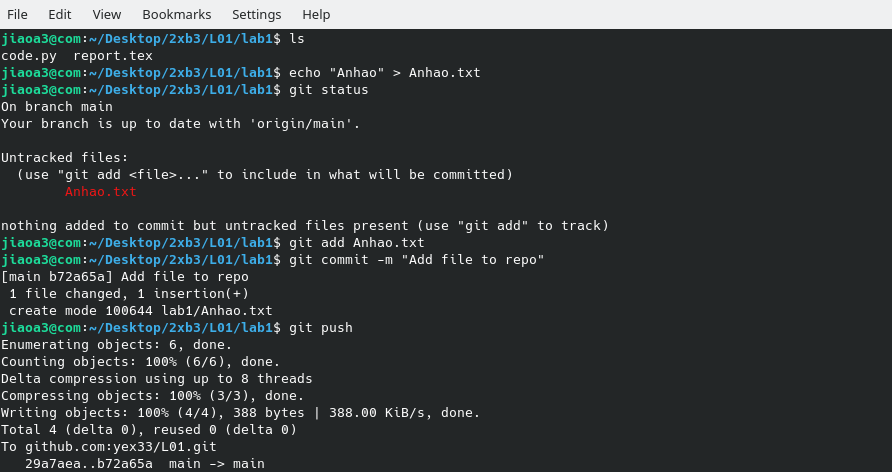
\includegraphics[width=\textwidth]{e1m1}
    \caption{Member 1}
  \end{figure}
  \begin{figure}[H]
    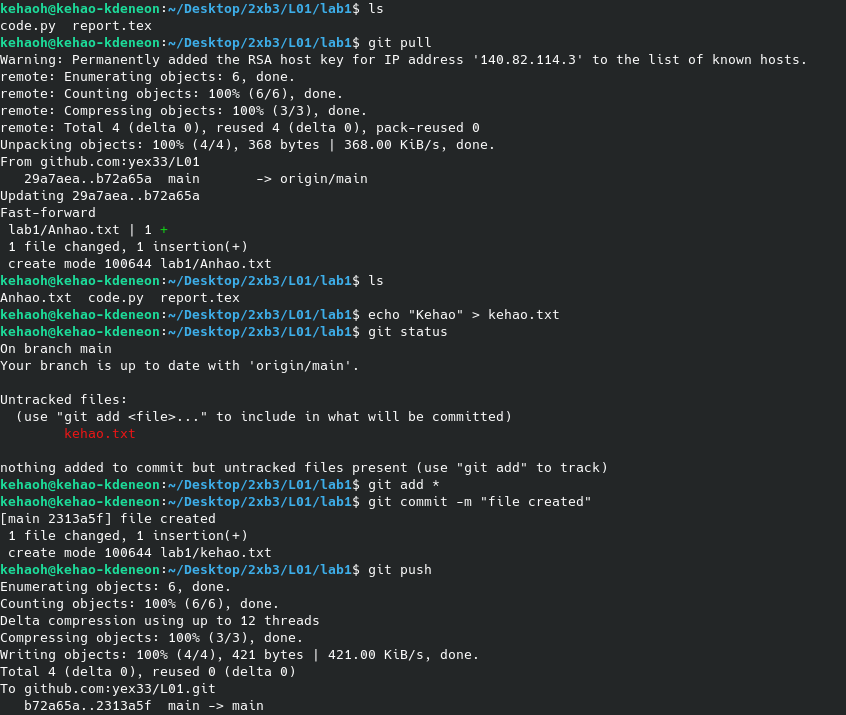
\includegraphics[width=\textwidth]{e1m2}
    \caption{Member 2}
  \end{figure}
  \begin{figure}[H]
    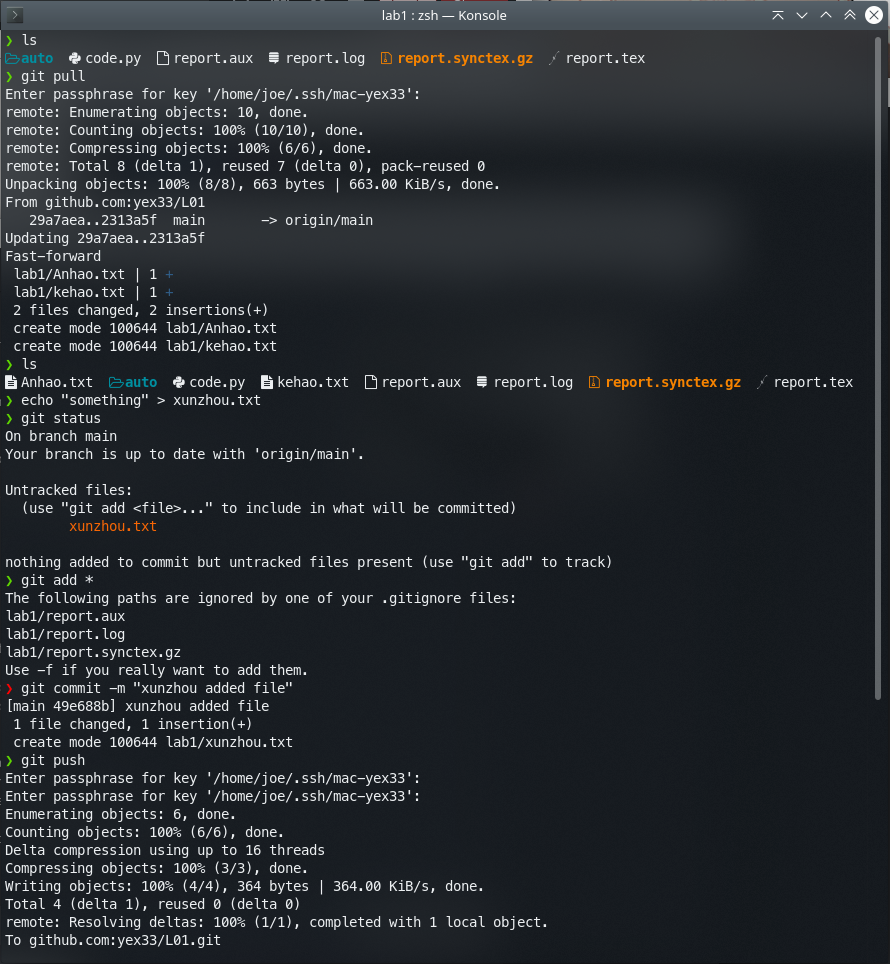
\includegraphics[width=\textwidth]{e1m3}
    \caption{Member 3}
  \end{figure}

  \section{Experiment 2 Screenshot}
  \begin{figure}[H]
    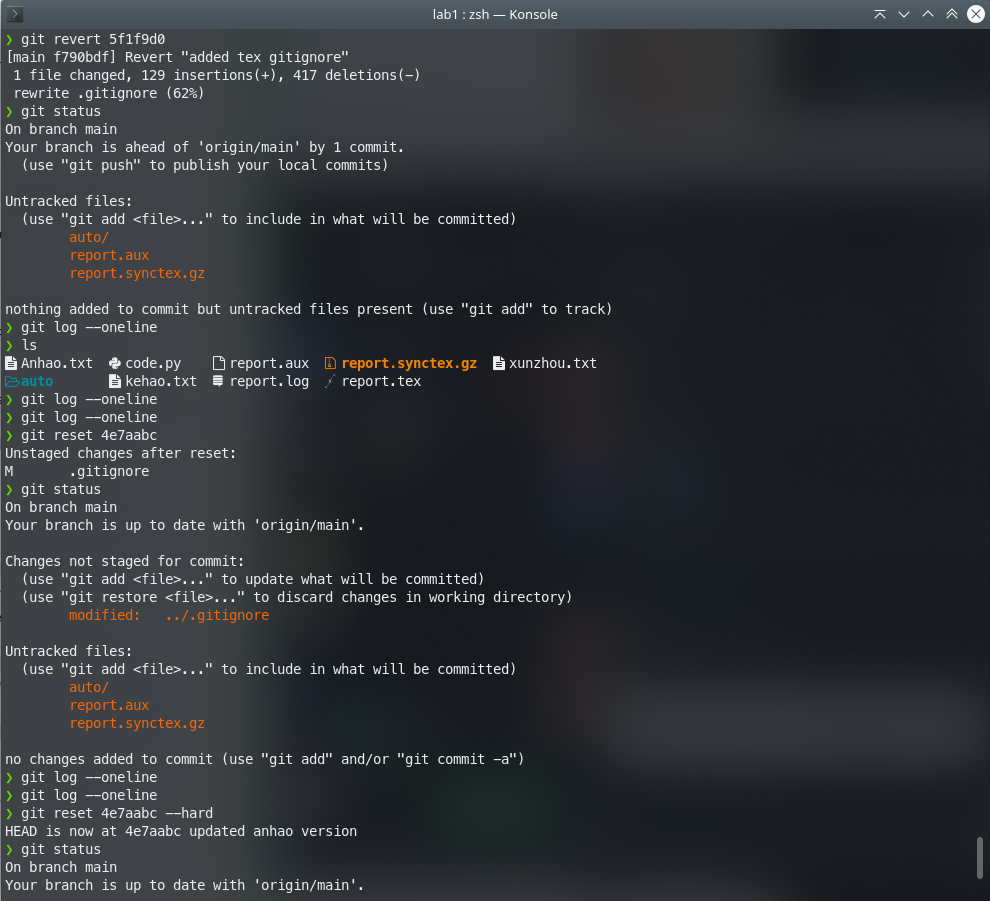
\includegraphics[width=\textwidth]{e2}
  \end{figure}

\end{appendices}
\end{document}
